\chapter{Artificial Neural Networks}
    This chapter provides the reader with background information on neural networks, focusing on the architectures and optimisation techniques used in this research. 
    
    The concept behind a neural network is formed from how neurons function within the human brain. It is built from the idea of an artificial neuron called a perceptron, which was developed in the 1950s-60s, by \citeauthor{perceptron_paper}. His work was inspired by a neurophysiologist named Warren McCulloch, and Walter Pitts, a mathematician, who published a paper which is now considered to be one of the foundational components that shaped artificial intelligence and cognitive science. They introduced the concepts of logical (threshold) neurons and neural networks which can be represented in a feedforward structure; see \cite{McCulloch1943}. 
    
    \section{Feedforward neural networks}
        Feedforward networks are primarily used for supervised\footnote{For a given input object, X, the desired output y is known.} learning tasks, where the data is neither sequential or time-series dependent. These networks contain a large number of computational units called neurons. These neurons are arranged into a layered structure, where the first layer is called the input layer, the intermediates are known as the hidden layers, and the final is called the output layer.  A network can have an arbitrary number of hidden layers; networks with many hidden layers are called deep neural networks. In a given layer, each neuron is connected to every neuron in the next layer. These connections enable information to flow through the network in a feedforward nature. 
        
        \subsection{Perceptrons}
        A neural network, in its most basic form, consists of a single neuron with no hidden layers, only an input layer, and an output layer. This is a type of supervised learning model, outlined by \cite{perceptron_paper}, and is referred to as a Perceptron.  This type of network is used for the classification of linearly separable data, i.e. patterns that can be separated with a single hyperplane\footnote{We refer the reader to \cite{hyperplane} for a detailed explanation of hyperplanes.}. A perceptron takes as input several variables, $x _1,x _2,...,x _m$ and produces a single output. Each input has an associated synaptic weight variable, $w _1,w _2,...,w _m$, and bias, $b$, both of which are adjusted and learned during training. 

        Consider the formula for $v$: 
        \begin{equation} \label{percetron_linear_transformation}
            v = \displaystyle\sum_{i=1}^{m} w_i x_i + b \quad ,
        \end{equation} 

        the value of $v$ is not bounded, it can be any value ranging from $-\infty$ to $\infty$. However, the goal of a perceptron is to correctly classify the inputs into one of two classes, $l _0$ or $l _1$. We therefore apply a decision rule, which acts as the activation function (discussed further in \ref{activation_functions}),  in order to define the output $y$. An example would be:
        
        \begin{equation} \label{simple_non_linear_transformation}
            y = 
                \begin{cases}
                    0  & \quad $if$ \quad \displaystyle\sum_{i=1}^{m} w_i x_i + b \quad \leq \quad 0 \quad, \\
                    1  & \quad $if$ \quad \displaystyle\sum_{i=1}^{m} w_i x_i + b \quad > \quad 0 \quad. \\
                \end{cases}
        \end{equation} 

        \vspace{20pt}

        \subsection{Multi-layer perceptron}
        A multi-layer perceptron (MLP) is a type of feedforward neural network, which contains more than one perceptron. MLPs contain an arbitrary number of hidden layers and are well suited to non-linear classification tasks. \cite{continuous_function_mapping} showed that multi-layer perceptron networks are capable of approximating any continuous function to any accuracy, provided there be enough hidden units/layers. This type of network is trained with Stochastic Gradient Descent (SGD) using a process called back-propagation to update the gradients and biases, discussed later in section \ref{gradient_descent} \& \ref{backprop}. We will be concerned with only this type of neural network for the rest of the thesis unless explicitly stated otherwise.  

            
        
    \section{Activation functions} \label{activation_functions}
        Activation functions are vital in neural networks; they decide if the neuron should be activated or not. The equation in \ref{simple_non_linear_transformation} shows that these functions can act as decision rules where the inputs are mapped to outputs which are commonly bounded between the range -1 and 1. More formally, there exists a non-linear mapping between the inputs to an activation function and the bounded output. Without this non-linearity, multiple layers would be equivalent to a single layer within the network. A critical feature of an activation function is that it must be fully differentiable, meaning we can find the slope of the curve at any point. This is important because the value of the derivative is used as a multiplier to update the weights of the network during backpropagation while training. 
        
        There are three main problems to consider when selecting an activation function, these are:
        
        \begin{enumerate}
            \item The vanishing gradient problem\footnote{Over time the neurons in the early layers have smaller and smaller gradients, meaning that they are the slowest to train.};
            \item Zero-centring;
            \item Computational requirement.
        \end{enumerate}
        
       
        
        \noindent We will now introduce three different types of activation functions. 
    
        \subsection{Sigmoid} \label{sigmoid}
            The sigmoid activation function is bounded between (0,1), and is defined as:
            
            \begin{equation}
                \sigma(x) = \frac{1}{ 1 + e^{-x} } \quad.
            \end{equation}
             
            \vspace*{1cm}
            
            \noindent The function and its derivative are shown in figure \ref{fig:sigmoid}. 
            
            \begin{figure}[H]
                \begin{subfigure}{0.5\textwidth}
                  \centering
                  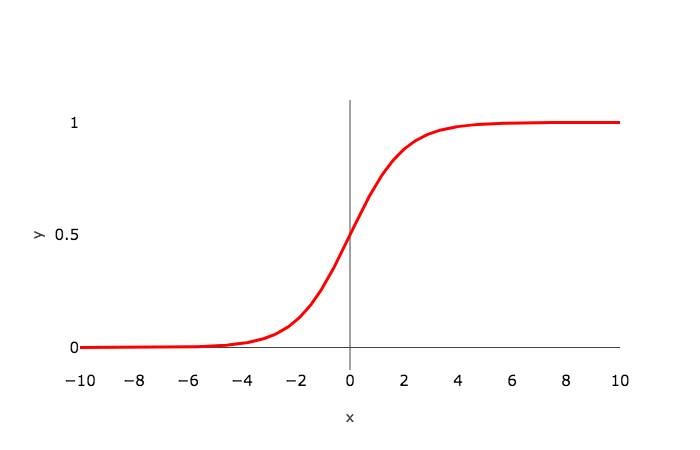
\includegraphics[width=1.0\linewidth]{Images/sigmoid.png}
                  \caption{$sigmoid$}
                  \label{fig:sig}
                \end{subfigure}%
                \begin{subfigure}{0.5\textwidth}
                  \centering
                  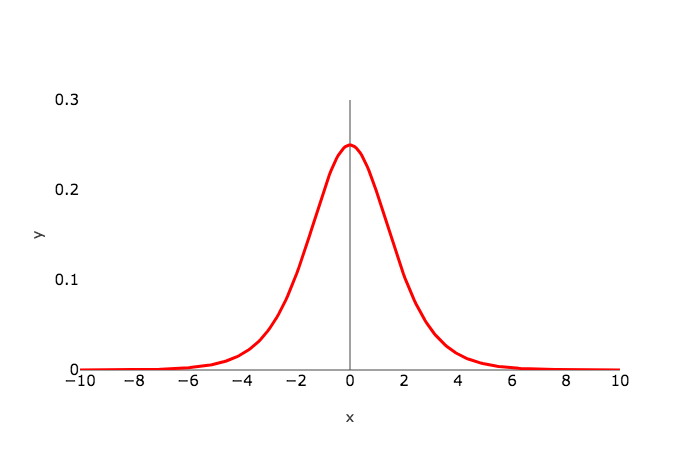
\includegraphics[width=1.0\linewidth]{Images/dsigmoid.png}
                  \caption{$sigmoid \, \, derivative$}
                  \label{fig:sig_div}
                \end{subfigure}
                \caption{Sigmoid Activation Function}
                \label{fig:sigmoid}
            \end{figure}
            
            The sigmoid function suffers from the vanishing gradient problem, as explained by \cite{activation_funcA}. The sigmoid graph (\ref{fig:sig}) shows that the gradients near the asymptotes tend towards zero. This tendency is confirmed by looking at the derivative (\ref{fig:sig_div}), which approaches 0 for large negative or large positive values. The problem with this is that, as mentioned previously, the value of the derivative is used to update the network during backpropagation. We can see that the derivative of the sigmoid function is bounded between (0, 0.25]. As a consequence, the update parameters of the network will continue to get smaller and smaller until learning stops altogether. Note that neurons with tiny weights, whereby no more learning can occur, are referred to as 'saturated' or 'dead' neurons.

            The sigmoid activation function is not zero-centered. This characteristic is undesirable since it is possible for neurons in later layers to receive input that is either all positive or all negative. This fluctuation can introduce 'zig-zag' dynamics, where a path through the network switches from positive to negative values between each layer during optimisation, as explained by \cite{activation_funcA}. 
            
            The sigmoid function uses the exponential function, $e^{-x}$, which is computationally an expensive function in comparison to other non-linear activations e.g. ReLU. 
            
            
        \subsection{Tanh}
            The tanh activation function is bounded between (-1,1). The function and it's derivative are shown in figure \ref{fig:tanh}. 
            \begin{figure}[H]
                \begin{subfigure}{0.5\textwidth}
                  \centering
                  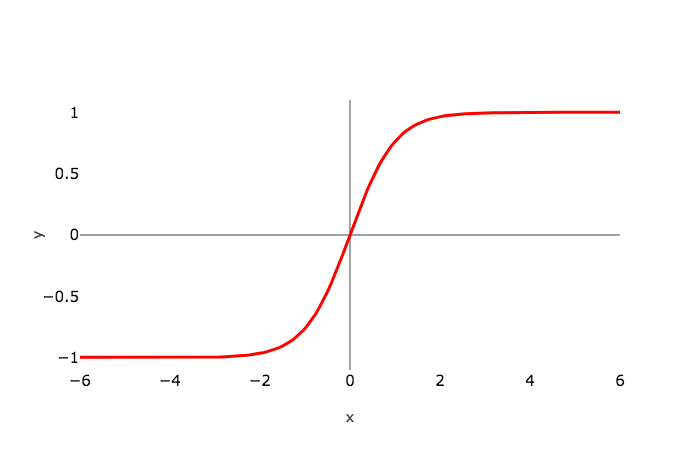
\includegraphics[width=1.0\linewidth]{Images/tanh.png}
                  \caption{$tanh(x)$}
                  \label{fig:tanh}
                \end{subfigure}%
                \begin{subfigure}{0.5\textwidth}
                  \centering
                  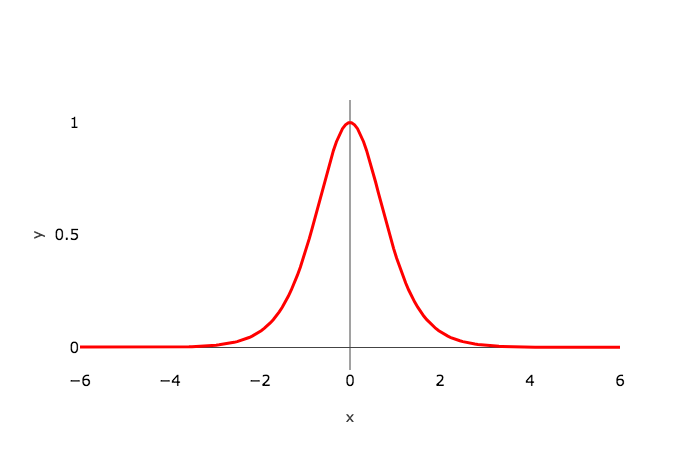
\includegraphics[width=1.0\linewidth]{Images/dtanh.png}
                  \caption{$tanh(x) \, \, derivative$}
                  \label{fig:tanh_div}
                \end{subfigure}
                \caption{Hyperbolic Tan Activation Function}
                \label{fig:tanh}
            \end{figure}

            Similarly, the tanh function also suffers from the vanishing gradient problem. From the graph (\ref{fig:tanh}), it can be seen that the gradients near the asymptotes tend towards zero. This characteristic is confirmed by looking at the derivative graph (\ref{fig:tanh_div}), which tends to 0 for large negative or large positive values. However, in contrast to the sigmoid function, we see that the derivative of tanh is bounded between (0, 1]. When this is combined with the fact that tanh is zero-centered, it results in the function providing stronger gradients during training. The zero-centre means that negative/positive inputs will be mapped strongly in the negative/positive direction; see \cite{activation_funcB}. However, for large positive or large negative values, the output still tends towards 0, and as such is still susceptible to the vanishing gradient problem. 
            
            The tanh function also uses the exponential function, $e^{-x}$, which, as mentioned in section \ref{sigmoid}, is computationally an expensive function in comparison to other non-linear activation's e.g. ReLU.
        
        \subsection{ReLU}
            The ReLU activation function is bounded between [0,$\infty$), and is defined as:
            
            \begin{equation}
                f(x) = max(0,x) \quad.
            \end{equation}
            
            The function and its derivative are shown in figure \ref{fig:relu}.  
            
            \begin{figure}[H]
                \begin{subfigure}{0.5\textwidth}
                  \centering
                  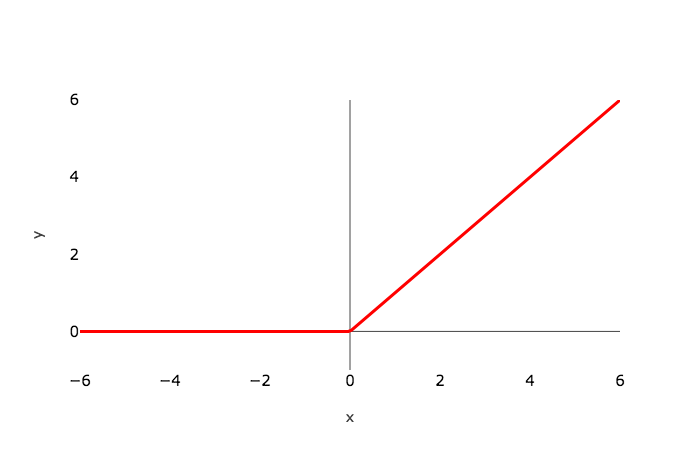
\includegraphics[width=1.0\linewidth]{Images/relu.png}
                  \caption{$relu$}
                  \label{fig:reluNorm}
                \end{subfigure}%
                \begin{subfigure}{0.5\textwidth}
                  \centering
                  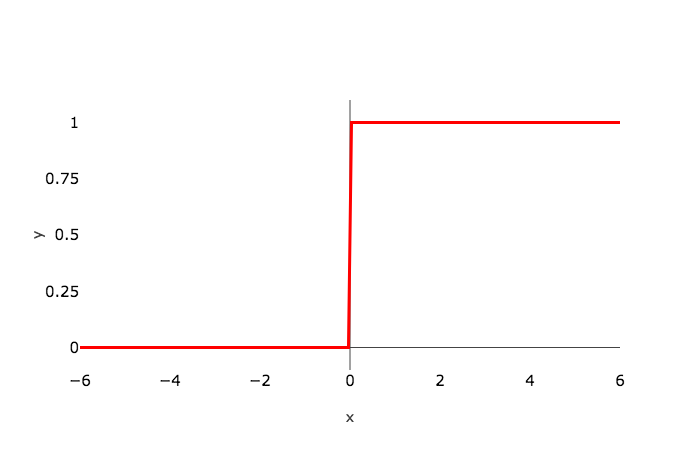
\includegraphics[width=1.0\linewidth]{Images/drelu.png}
                  \caption{$relu \, \, derivative$}
                  \label{fig:reluDer}
                \end{subfigure}
                \caption{ReLU Activation Function}
                \label{fig:relu}
            \end{figure}
            
            ReLU is the most commonly used activation function and is the one we select to use in our network, as it does not suffer directly from the vanishing gradient problem. As can be seen in the graph (\ref{fig:reluNorm}), for any values where $x < 0$ the output is 0, and for any values where $x > 0$ the output is $x$. This simple threshold rule makes ReLU very computationally efficient, in comparison to the tanh and sigmoid function. The derivative of ReLU (\ref{fig:reluDer}) allows the network to learn without neuron saturation, where the output is 1 for large values of $x$ and 0 for negative values; see \cite{activation_funcA}. Although ReLU is not zero-centred, as seen in figure \ref{fig:reluNorm}, this problem can be overcome by regularisation techniques which are discussed in more detail in section \ref{sec: regularise}. 
            
        % https://www.learnopencv.com/understanding-activation-functions-in-deep-learning/
        

        

    \section{Loss function} \label{loss_function}
        A loss or error, function $J(p, \hat{p})$ is calculated by computing the difference between the predicted output $\hat{p}$ and actual output $p$. The output of a loss function is used to update the weights and biases in a neural network using a process called Back-Propagation as discussed later in section \ref{backprop}. There exist many different loss functions which produce different results given the same values for $\hat{p}$ and $p$. Selecting a loss function is highly dependent on the type of machine learning problem, be it regression or classification.
        
        \subsection{Cross-Entropy Loss}
            Cross-Entropy, or log, loss is a commonly used loss function for classification problems. It is calculated using the formula: 
            
            \begin{equation} \label{cross_entropy_formula}
                CrossEntropy(p, \hat{p}) = -\sum_{\mathclap{i}}^{} p_i \log{\hat{p_i}} \quad,
            \end{equation}
            
            where $\hat{p}$ is the predicted output, and $p$ is the actual output.
           
            \vspace*{0.3cm}

            The loss function imposes an exponentially increasing error as the predicted output and the actual output diverge. Similarly, as the difference between the predicted output and actual output is reduced, the output of the loss function becomes exponentially smaller.  
            
            

        \subsubsection{Softmax Cross-Entropy Loss}
            The Softmax Cross-Entropy loss is similar to Cross-Entropy loss with the addition of a Softmax activation layer, where the output of the Softmax layer is used as input to the Cross-Entropy loss function. 
            
            \begin{equation} \label{softmax_formula}
                Softmax(x_i) = \frac{e^{x_i}}{\sum_{\mathclap{j}}^{} e^{x_j}} \quad,
            \end{equation}
            
            where $x_i$ is the $i^{th}$ output of final layer.
            
            \vspace*{0.3cm}
            
            The Softmax layer, as shown in formula \ref{softmax_formula}, is advantageous as it introduces non-linearity by producing a probability distribution whose sum is equal to 1, i.e. it outputs the probability of each class. Therefore this type of loss function is typically suited to multi-class classification problems, where each input belongs to exactly 1 class. Our classification task, as defined fully in section \ref{default_prediction}, fits this criteria. We therefore choose the Softmax Cross-Entropy loss function in our network.
            
            % , and ${\sum_{\mathclap{j}}^{}}$ represents the sum of over all outputs in the final layer. 
            
        % \subsubsection{Sigmoid Cross-Entropy Loss}
        %     The Sigmoid Cross-Entropy loss is similar to Softmax Cross-Entropy loss with the Softmax activation layer replaced by the Sigmoid activation layer. The Sigmoid layer, formula in \ref{sigmoid_formula}, introduces non-linearity by producing a marginal probability distribution where each probability is between 0 and 1. Therefore this type of loss function is typically suited to multi-label classification problems, where an input can belong to multiple classes.
            
        %     \begin{equation} \label{sigmoid_formula}
        %         Sigmoid(x) = \frac{1}{1 + e^{-x}} \quad.
        %     \end{equation}

        
    \section{Training neural networks}
        This section is a technical overview that outlines the training steps involved when training a feed forward multi-layered neural network. It also introduces a number of specific optimisation techniques that we implement in the final model. The mathematical formulae in this section are based on the explanations from the book Neural Networks and Deep Learning, \cite{book_king_NN}.
    
        \subsection{Gradient Descent} \label{gradient_descent}
            Gradient descent, or steepest descent, is a type of algorithm used to find the minimum of a function. In the case of a neural network, gradient descent is used to minimise the loss function, the difference between the predicted output $\hat{p}$ and actual output $p$. 
            This objective is achieved by iteratively updating the weights and biases by minimising the gradient of the loss function with respect to both the weights and biases. We can define the general update rule for a given weight as:
            
            \begin{equation} \label{update_rule}
                w_{kj} = w_{kj} - \eta \Delta w_{kj} \quad ,
            \end{equation}
            
            where $w_{kj}$ is the weight associated with the $j^{th}$ neuron in layer $l$ and $k^{th}$ neuron in layer $l + 1$, and where $\eta$ is the learning rate. Unfortunately computing $ \Delta w_{kj}$ is not trivial and is discussed in more depth in Section \ref{backprop}.
            
        \subsection{Mini-Batch Gradient Descent} \label{mini_batch}
            In order to find the exact gradient of the loss function with respect to the weights and biases, it is necessary to calculate the sum of gradient over all data points in the training set. Operating large datasets, as we are in this thesis (see section \ref{data_format}), means that this calculation is computationally expensive and would take an unfeasible amount of time to train. We adopt Mini-Batch Gradient Descent, which calculates an approximation of the gradient based on a subset (mini-batch) of the dataset. The equation is defined as follows:
            
            \begin{equation} \label{eq:mini_batch}
               \Delta w_{kj} = \frac{ 1 } { b } \sum_{\mathclap{i=0}}^{b} \Delta w_{kj} \quad,
            \end{equation}
            where $b$ is the size of the mini-batch, and $\Delta w_{kj}$ is the average gradient over all $b$ samples. During training, the algorithm will iterate over the dataset a specified number of times, where a single cycle of the entire dataset is known as 1 epoch. Note that it is important to randomly shuffle the dataset after each epoch to prevent repeating update cycles.  
                

        \subsection{Learning rate} \label{learning_rate}
            The learning rate $\eta$ is used to control how much the weights should be adjusted with respect to the gradient of the loss function. Small learning rates will take longer to minimise the loss function and have a higher probability of converging in a local minimum. Conversely, high learning rates have a higher probability of not converging or even diverging. 
            
            Adaptive learning rates, where the rate reduces over time, are an approach to mitigate these problems. We define an adaptive learning rate using the following formula: 
            
            \begin{equation} \label{lr_adaptive}
                \eta = \frac{ \eta } { 1 + k t } \quad,
            \end{equation}
            where $t$ is the number of epochs, and $k$ is an arbitrary constant. 
        
        \subsection{Momentum} \label{momentum}
            Momentum is a technique we adopt in this work. It is used to help prevent the network getting stuck in a local minimum. With momentum $m$, the weight update rule is defined as: 
            \begin{equation} \label{SGD}
               \Delta w^{t}_{kj} = \eta \Delta w^{t}_{kj} + m \Delta w^{t-1}_{kj} \quad,
            \end{equation}
            where $m$ is a parameter between 0 and 1 (determined by trial and error), and $t$ is the step number for gradient descent method. Momentum uses a fraction of the previous weight gradient, $\Delta w^{t-1}_{kj}$, to determine the current gradient value. This calculation means that when the gradient is pointing in the same direction, the update factor will be larger, gaining momentum. It is therefore necessary to reduce the learning rate $\eta$ significantly when using a momentum value close to 1. 
            
        \subsection{Backpropagation} \label{backprop}
            A feedforward neural network learns in two stages, the forward pass and backwards pass. The forward pass refers to the calculation process through all neurons from the first to the last layer, producing the predicted output $\hat{p}$. The backward pass refers to a calculation process through all neurons from the last to the first layer, where the weights and biases are updated based on how different the predicted output $\hat{p}$ is from the actual output $p$.
            
            The backpropagation algorithm is a special case of automatic differentiation and is the most common method for updating neural networks in the backward pass. The objective of the algorithm is to update the weights and biases in each layer by computing the partial derivative of the cost function $J$ with respect to each weight $w$ and bias $b$ in a neural network. In a multi-layer perceptron, backpropagation allows the error to propagate back through the network layer by layer, updating the weights and biases accordingly. 

            This section will evaluate how the weights are updated using the Mean Squared Error (MSE) loss function,  $J$. 
            
            First consider a multi-layer perceptron network with $l$ layers, where $\boldsymbol{a^l}$ is the output vector of the activation functions at layer $l$, $\boldsymbol{b^l}$ is the biases for the neurons in layer $l$, and $\boldsymbol{W^l}$ is the weight vector associated with layers $l$ and $l+1$.
            
            For the forward pass of the network we have: 
            \begin{equation} \label{backpropagation_formula}
                \boldsymbol{a^l} = \sigma^{l}{ (\boldsymbol{W^l} \cdot \boldsymbol{a^{l-1}} +  \boldsymbol{b^l})  }
            \end{equation}
            where $\sigma^{l}$ represents an activation function at layer $l$. 
            
            We denote $z^{l}_{k}$ to represent the input sum to the activation function of the $k^{th}$ neuron in layer $l$:
            
            \begin{equation} \label{input_sum_neuron2}
                z^{l}_{k} = \sum_{\mathclap{j}}^{} w^{l}_{kj} a^{l-1}_{j} + b^{l}_{k}
            \end{equation}
            where $w^{l}_{jk}$ is the weight associated with the $j^{th}$ neuron in layer $l$ and $k^{th}$ neuron in layer $l + 1$, and $b^{l}_{k}$ is the bias associated with the $k^{th}$ neuron in layer $l$. 
            
            We rewrite the forward pass as: 
            \begin{equation} \label{activation_layer_formula}
                a^{l}_{k} = \sigma^{l}{ (z^{l}_{k})  }
            \end{equation}
            where $\sigma^{l}$ represents an activation function at layer $l$.

            Consider a loss, or error function $J$. The error function in classic backpropagation is Mean Squared Error (MSE), which we denote as:
            \begin{equation} \label{MLE_Formula}
               J =\sum_{\mathclap{j=0}}^{n-1} (a^{l}_{j} - y_{j})^2 \quad .
            \end{equation}
            
            We denote the derivative of the loss function $J$ with respect to the weights as:
            
            \begin{equation} \label{chain_rule_A}
                \frac{ { \partial J } } { { \partial w^{l}_{kj} } } 
                \,\, = \,\,  
                % { \sum_{\mathclap{k}}^{} 
                    {
                        { \frac{ { \partial J } } { { \partial z^{l}_{k} } } }
                        { \frac{ { \partial z^{l}_{k} } } { { \partial w^{l}_{kj} } } }
                    }
                % }
                \,\, = \,\,  
                % { \sum_{\mathclap{k}}^{} 
                    {
                        { \frac{ { \partial J } } { {  \partial a^{l}_{k} } } }
                        { \frac{ { \partial a^{l}_{k} } } { { \partial z^{l}_{k} } } }
                        { \frac{ { \partial z^{l}_{k} } } { { \partial w^{l}_{kj} } } }
                    }
                % }
                \,\, = \,\,  
                \Delta w_{kj} \quad .
            \end{equation}
            
            \vspace*{0.5cm}
            
            
            
            We consider the first term $\frac{ { \partial J } } { {  \partial a^{l}_{k} } }$ from \ref{chain_rule_A}, using the equation for $J$ defined in \ref{MLE_Formula}:
            \begin{align}
                \frac{ { \partial J } } { { \partial a^{l}_{j} } } \,
                    & = \, 
                        \frac{ { \partial } } { { \partial a^{l}_{j} } } \left( \sum_{\mathclap{j=0}}^{n-1} (a^{l}_{j} - y_{j})^2 \right) 
                    \nonumber \\
                % \frac{ { \partial } } { { \partial a^{l}_{j} } } \left( \sum_{\mathclap{j=0}}^{n-1} (a^{l}_{j} - y_{j})^2 \right) 
                    & = \, 
                        \frac{ { \partial } } { { \partial a^{l}_{j} } } 
                            \left( 
                                (a^{l}_{0} - y_{0})^2 \, \, + \, \,
                                \dots \, \, + \, \,
                                (a^{l}_{j} - y_{j})^2 \, \, + \, \,
                                \dots 
                                % \dots \, \, + \, \,
                                % (a^{l}_{n-1} - y_{n-1})^2  
                            \right) 
                        \nonumber \\
                    & = \, 
                        \frac{ { \partial } } { { \partial a^{l}_{j} } }  \left( (a^{l}_{0} - y_{0})^2 \right)  \, \, + \, \,
                        \dots \, \, + \, \,
                        \frac{ { \partial } } { { \partial a^{l}_{j} } } \left( (a^{l}_{j} - y_{j})^2 \right) \, \, + \, \,
                        \dots 
                        % \dots \, \, + \, \,
                        % \frac{ { \partial } } { { \partial a^{l}_{j} } } \left( (a^{l}_{n-1} - y_{n-1})^2 \right) 
                        \nonumber \\
                    & = \, 
                        2(a^{l}_{j} - y_{j}) \quad .
                        \nonumber \\
            \end{align}
            
            We consider the second term $\frac{ { \partial a^{l}_{k} } } { { \partial z^{l}_{k} } }$ from \ref{chain_rule_A}, using the equation for $a^{l}_{k}$ defined in \ref{activation_layer_formula}:
            \begin{align}
                \frac{ { \partial a^{l}_{j} } } { { \partial z^{l}_{j} } } \,
                    & = \, 
                        \frac{ { \partial } } { { \partial z^{l}_{j} } } \left( \sigma^{l}{ (z^{l}_{j}) } \right) 
                    \nonumber \\
                    & = \, 
                        {\sigma^{\,l}}\,^{'}{\,\, (z^{l}_{j}) } \quad .
                        \nonumber \\
            \end{align}
            
            We consider the third term $\frac{ { \partial z^{l}_{k} } } { { \partial w^{l}_{kj} } }$ from \ref{chain_rule_A}, using the equation for $z^{l}_{k}$ defined in \ref{input_sum_neuron2}:
            \begin{align}
                \frac{ { \partial z^{l}_{k} } } { { \partial w^{l}_{kj} } } 
                    & = \, 
                        \frac{ { \partial } } { { \partial w^{l}_{kj} } } \left( \sum_{\mathclap{i}}^{} w^{l}_{kj} a^{l-1}_{j} + b^{l}_{k} \right) 
                    \nonumber \\
                    & = \, 
                        \frac{ { \partial } } { { \partial w^{l}_{kj} } } 
                        \left( 
                            (w^{l}_{k0} a^{l-1}_{0} + b^{l}_{k}) \, \, + \, \, 
                            \dots \, \, + \, \,
                            (w^{l}_{kj} a^{l-1}_{j} + b^{l}_{k}) \, \, + \, \,
                            \dots
                        \right) 
                    \nonumber \\
                    & = \, 
                        \frac{ { \partial } } { { \partial w^{l}_{kj} } } (w^{l}_{k0} a^{l-1}_{0} + b^{l}_{k}) \, \, + \, \, 
                        \dots \, \, + \, \,
                        \frac{ { \partial } } { { \partial w^{l}_{kj} } } (w^{l}_{kj} a^{l-1}_{j} + b^{l}_{k}) \, \, + \, \,
                        \dots
                    \nonumber \\
                    & = \, 
                        a^{l-1}_{j} \quad .
                    \nonumber \\
            \end{align}
            
            
            We have now evaluated all three terms from \ref{chain_rule_A}, we denote the gradient with respect to the weights for the MSE loss function to be:
            
            \begin{align} \label{eq_weight_gradient}
                \Delta w_{kj} = \frac{ { \partial J } } { { \partial w^{l}_{kj} } }
                & = \,  
                % { \sum_{\mathclap{k}}^{} 
                    {
                        { \frac{ { \partial J } } { {  \partial a^{l}_{k} } } }
                        { \frac{ { \partial a^{l}_{k} } } { { \partial z^{l}_{k} } } }
                        { \frac{ { \partial z^{l}_{k} } } { { \partial w^{l}_{kj} } } }
                    }
                % }
                \nonumber \\
                & = \,
                    \left( 2(a^{l}_{j} - y_{j}) \right) \,\, \left( \sigma'^{\,\,l}{\,(z^{l}_{j}) } \right) \,\, \left( a^{l-1}_{j} \right) \quad .
            \end{align}
            
            We can use the formula for $\Delta w_{kj}$ in equation \ref{eq_weight_gradient} to update the weights as described in Section \ref{gradient_descent}. The update rule under the MSE loss function would be:
            
            \begin{align}
                w_{kj} 
                & = \,  
                 w_{kj} - \eta \Delta w_{kj} 
                \nonumber \\
                & = \,
                     w_{kj} - \eta \left( 2(a^{l}_{j} - y_{j}) \right) \,\, \left( \sigma'^{\,\,l}{\,(z^{l}_{j}) } \right) \,\, \left( a^{l-1}_{j} \right) \quad . 
            \end{align}
            
    \subsection{Weight Initialisation} \label{weight_initalisation}             
        Weight initialisation is an important consideration when training a deep multi-layered neural network. The initial weight values can significantly affect both the speed and optimality of convergence during stochastic gradient descent. That is, if the weight values are small, the output of the loss function will also be small, resulting in small updates to the network. In turn, reducing the speed of convergence and increases the probability of converging in a sub-optimal minimum.
        
        The network in this paper uses the Xavier initialisation algorithm, which is a popular weight initialisation technique. The objective of the algorithms is to produce weight values that follow a distribution (typically Gaussian or uniform), with zero mean and a specified variance, across all the neurons in the layer. We refer the reader to the original paper by Xavier Glorot, 2010 for more implementation details \cite{xavier_weight_initalisation}. 
        
\section{Layers}
    \subsection{Batch Normalisation} \label{batch_norm_sec}
        Batch Normalisation is a common technique for improving stability and the performance of a neural network. Since it's introduction by \cite{batch_normalisation}, it has quickly become a standard optimisation technique when training deep neural network. It works by standardising the input layer, x, by subtracting the mean and dividing by the standard deviation. The standardised layer, z, is multiplied by an arbitrary parameter g, and an arbitrary parameter b is added to the resulting product. 

        % \vspace{20pt} \noindent The formula for Batch Normalisation for a layer with d-dimensional input $x = (x^{(1)} , x^{(2)}. . . x^{(d)})$, is shown in equation \ref{eq_BN}.
        %     \begin{equation} \label{eq_BN}
        %         BN(x^{(k)}) = ( z^{(k)} * g^{(k)} ) + b^{(k)},  \quad \textrm{and} \quad  z^{(k)} = \frac{x^{(k)} - E[x^{(k)}]}{Var[x^{(k)}]}
        %     \end{equation}
        %     \begin{adjustwidth}{2.5em}{0pt}
        %         Where:
        %         \begin{itemize}[label=]
        %             \item $x$: is the input layer
        %             \item $z$: is the standardised output of the input layer. 
        %             \item $g, b$: are learnt parameters
        %         \end{itemize}
        %     \end{adjustwidth}
    
            
        % \vspace{20pt} \noindent
        The batch normalisation process means that the weights within the network do not become imbalanced with extremely high or low values since the standardisation is included in the SGD process. The learned parameters $g, b$ mean that the \textit{Covariate Shift}\footnote{The change in the distribution of network activation's due to a change in network parameters} between the layers is reduced. The backpropagation algorithm then allows the network to learn by how much each layers' activation should be normalised. 
        
        The addition of batch normalisation can significantly increase the speed at which training occurs, and reduce the probability that a particular batch cycle will over influence the training process. It allows for the use of higher learning rates as the output values do not deviate significantly from the mean, reducing the likelihood of an exploding or vanishing gradient problem as well as getting stuck in a sub-optimal minimum.

\section{Regularisation} \label{sec: regularise}
    
    Regularisation is a very important technique in deep learning to prevent overfitting\footnote{A problem where the classifier learns features that are specific to the training data and therefore performs badly on unseen validation data.}. In general, regularisation reduces high valued weights in the network, reducing the flexibility of the model and making it less likely to fit noise within the training data. There exists a variety of regularisation strategies, each with their advantages and drawbacks; this section will give an overview of some of these techniques. We inform the reader that these techniques are analysed in further detail and compared with batch normalisation in the results section (\ref{BN_l2_drop_results}).

    \subsection{Dropout} 
        Dropout is a type of regularisation technique that was first introduced by \cite{dropout_hinton}. The literature explains that dropout is where "each hidden unit is randomly omitted from the network with a probability." It is later stated that dropout can be used to reduce overfitting and can be viewed as a very efficient way of performing model averaging within the network. 
        
    \subsection{$L^2$ Regularisation} \label{l2_regularisation}
        $L^2$ Regularisation, or weight decay, is a regularisation strategy that moves the weights closer to the origin\footnote{The weights could be regularised towards any point in space and still achieve a regularising effect.} by adding a regularisation term. \cite{regularising_comparison} showed that large weights are more often found in networks where overfitting occurs, $L^2$ regularisation attempts to mitigate this by keeping the weights small. 
        
        $L^2$ regularisation is achieved by modifying the loss function and adding a weight penalty, which causes larger weights within the network to have a higher loss. The equation for $L^2$ regularisation is the following:
        
        \begin{equation} \label{l2_equation}
            J = J_0 + \frac{\lambda}{2n} \sum_{\mathclap{l}}^{} \boldsymbol{W^{[l]}}^2 \quad,
        \end{equation}
        % \boldsymbol{W^l}
        where $J_0$ is the unregularised cost function, n is the size of the training set and  $\boldsymbol{W^{[l]}}$ is the weight vector between layers $l$ and $l+1$. Note that a typical value for regularisation term, $\lambda$, falls within the range 0.01 to 0.05; as stated by \cite{regularising_comparison}.
        


\subsubsection{Conclusion}
    In this chapter we provided a detailed introduction to multi-layered feedforward neural networks. We introduced different types of activation functions, explaining both the advantages and drawbacks. We provided a technical explanation of back-propagation, the algorithm by which neural networks update their weights and biases relative to the chosen loss function. We discussed the importance of weight initialisation, its effect on the speed and optimality of convergence during stochastic gradient descent (SGD), and introduced the Xavier initialisation approach. We then explained how Batch Normalisation can increase the speed of convergence and reduce the \textit{Covariate Shift} during SGD. Finally, we introduced two Regularisation techniques, Dropout and $L^2$ Regularisation.


